Lektion-4-Vorspann

%\sttpLeserfuehrungMindMap{Bilder/Kapitel-3/Abb-3-1-MindMap-Leserfuehrung-Illustration-Modellierungsgegenstand.pdf}{Bilder/Kapitel-6/Abb-3-1-MindMap-Leserfuehrung-Modellierungsgegenstand_Software.pdf}

%%=====================================================================================

6.1.4 - Zoo

%*************** Sprechblaseninhalte ************
%\begin{itemize}[
%	label={\raisebox{-2mm}{
\includegraphics[scale=0.8]{Bilder/speech_balloon_green.pdf}}},
%	leftmargin=12mm,
%	]
%	\item Wir möchten die Besucherzahl des Zoos deutlich erhöhen.
%	\item Die Software soll den Zoo über die Region hinaus bekannt machen.
%	\item Die Software kann Tierpatenschaften verwalten. Die Nutzer sollen Patenschaften über das Internet buchen und abbestellen können. 
%	\item Der Zoo braucht ein Profil mit einem Alleinstellungsmerkmal.
%	\item Alle Zoobesucher sollen die Möglichkeit bekommen, Namen für neugeborene Tiere vorzuschlagen. 
%	\item Man kann Führungen durch den Zoo online buchen. 
%	\item Online Eintrittskarten für den Zoo verkaufen
%	\item Es sollen umfangreiche Informationen über den Zoo und seine Tiere über das Internet zugänglich gemacht werden.
%	\item Den Bildungsauftrag des Zoos erfüllen
%	\item Zoo in der Region verankern, Bindung der Einwohner an den Zoo erhöhen, Identifizierung mit dem Zoo
%	\item Viel deutlicher herausstellen, dass wir viele besondere Tierarten haben, die es in anderen Zoos nicht gibt.
%	\item Umfangreiche Unterstützung der Besucher beim Besuchserlebnis
%	\item Unsere Website soll umfangreiche Informationen zu den Tieren bereitstellen. 
%	\item Trackingsystem der Besucher, um ihnen mitteilen zu können, wenn das Elefantenhaus oder das Affenhaus gerade zu stark besucht sind.
%	\item Ziel ist, den Zoo dauerhaft finanziell gut ausgestattet zu haben und ihm somit eine langfristige Perspektive zu bieten. 
%	\item Auf der Website auf Events wie die Ausleihe eines besonderen Tiers hinweisen
%	\item Die Besucher im Zoo über ihre Handys informieren, wenn in ihrer Nähe eine Fütterung startet
%	\item Warteschlangenverwaltung für den Streichelzoo
%\end{itemize}
%
%************** Ende ***********************
%
%- evtl. Wolkengrafik

%%=====================================================================================

Kapitel 6.2.1.2

%TODO: kommt evtl. wieder rein
%Abbildung~\ref{fig:bestandteile_vision} zeigt die Bestandteile einer Vision.

%\begin{figure}
%	\centering
%	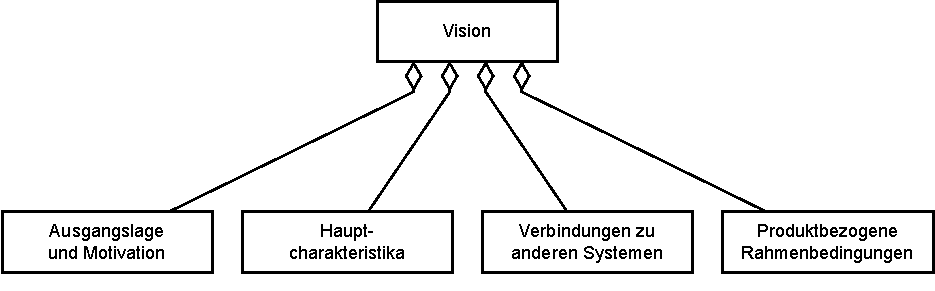
\includegraphics[width=\textwidth]{Bilder/Kapitel-6/bestandteile_vision.pdf}
%	\caption{Bestandteile einer Vision}
%	\label{fig:bestandteile_vision}
%\end{figure}

%%=====================================================================================

Kapitel 6.3.1

%\begin{center}
%	\begin{minipage}[c]{.35\linewidth} 
	%		\sttpAbbildungskasten{Bilder/Kapitel-6/UML-Diagramme-Kap-6-Leserfuehrung-Anwendungsfalldiagramm.pdf}{0.35}
	%	\end{minipage}
%	\hspace{.05\linewidth}% Abstand zwischen den beiden Bildern
%	\begin{minipage}[c]{.5\linewidth}
	%		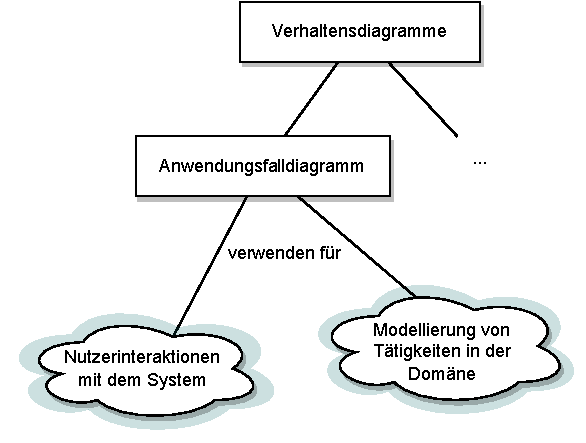
\includegraphics[width=\linewidth]{Bilder/Kapitel-6/UML-Diagramme-Kap-6-Anwendungsfalldiagramm.pdf}
	%	\end{minipage}
%\end{center}

%%=====================================================================================

